% AUTO-GENERATED by build/gen_corpus.py from literature/corpus.tsv -- do not hand-edit.
\begin{figure}[t]
\centering
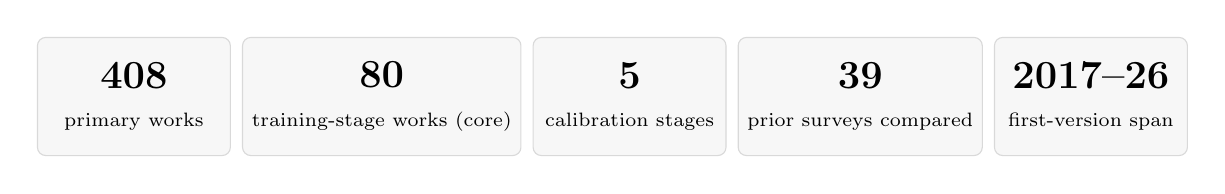
\begin{tikzpicture}
\matrix[column sep=4pt]{
\node[draw=black!15,fill=black!3,rounded corners=3pt,minimum width=2.45cm,minimum height=1.5cm,align=center] {\Large\bfseries 408\\[2pt]\scriptsize primary works}; & \node[draw=black!15,fill=black!3,rounded corners=3pt,minimum width=2.45cm,minimum height=1.5cm,align=center] {\Large\bfseries 80\\[2pt]\scriptsize training-stage works (core)}; & \node[draw=black!15,fill=black!3,rounded corners=3pt,minimum width=2.45cm,minimum height=1.5cm,align=center] {\Large\bfseries 5\\[2pt]\scriptsize calibration stages}; & \node[draw=black!15,fill=black!3,rounded corners=3pt,minimum width=2.45cm,minimum height=1.5cm,align=center] {\Large\bfseries 39\\[2pt]\scriptsize prior surveys compared}; & \node[draw=black!15,fill=black!3,rounded corners=3pt,minimum width=2.45cm,minimum height=1.5cm,align=center] {\Large\bfseries 2017--26\\[2pt]\scriptsize first-version span}; \\
};
\end{tikzpicture}\\[6pt]
\begin{tikzpicture}
\begin{axis}[xbar,bar width=10pt,width=0.84\textwidth,height=5.6cm,xmin=0,
  symbolic y coords={{X consumers and contract},{Theory and analysis},{S4 training},{S3 extra inference},{S2 prompt elicitation},{S1 post-hoc map},{S0 read-off}},ytick={{X consumers and contract},{Theory and analysis},{S4 training},{S3 extra inference},{S2 prompt elicitation},{S1 post-hoc map},{S0 read-off}},y dir=normal,
  nodes near coords,nodes near coords style={font=\footnotesize},xlabel={\footnotesize works},tick label style={font=\footnotesize},
  axis line style={black!45},xmajorgrids,grid style={black!8},enlarge x limits={upper,value=0.12}]
\addplot[fill=stS0,draw=none,bar shift=0pt] coordinates {(25,{S0 read-off})};
\addplot[fill=stS1,draw=none,bar shift=0pt] coordinates {(52,{S1 post-hoc map})};
\addplot[fill=stS2,draw=none,bar shift=0pt] coordinates {(54,{S2 prompt elicitation})};
\addplot[fill=stS3,draw=none,bar shift=0pt] coordinates {(121,{S3 extra inference})};
\addplot[fill=stS4,draw=none,bar shift=0pt] coordinates {(80,{S4 training})};
\addplot[fill=stTH,draw=none,bar shift=0pt] coordinates {(5,{Theory and analysis})};
\addplot[fill=stX,draw=none,bar shift=0pt] coordinates {(71,{X consumers and contract})};
\end{axis}
\end{tikzpicture}
\caption{\textbf{The corpus at a glance.} 408 primary works (451 references cited across the figures and tables), placed by the stage at which
calibration enters (Table~\ref{tab:definitions}); the X group holds works that consume the confidence or fix the output
contract, and the theory group holds analyses of training-stage calibration. 39 prior surveys are compared in
Table~\ref{tab:survey_compare}.}
\Description{Five stat cards (works, training-stage works, stages, prior surveys and year span) above a horizontal bar
chart of works per stage.}
\label{fig:corpus_overview}
\end{figure}
